\documentclass[a4paper, 12pt, twoside]{article}
\usepackage[T2A,T1]{fontenc}
\usepackage[utf8]{inputenc}
\usepackage[english, russian]{babel}
\usepackage{graphicx}
\usepackage[hcentering, bindingoffset = 10mm, right = 15 mm, left = 15 mm, top=20mm, bottom = 20 mm]{geometry}
\usepackage{multirow}
\usepackage{ctable}
\usepackage{lipsum}
\usepackage{amsmath, amstext}
\usepackage{siunitx}
\usepackage{subcaption}
\usepackage{wrapfig}
\usepackage{adjustbox}
\usepackage{enumerate, indentfirst, float}
\usepackage{capt-of, svg}
\usepackage{cmap} % Улучшенный поиск русских слов в полученном pdf-файле

\usepackage{pscyr} % Нормальные шрифты
\usepackage[normalem]{ulem} % для подчёркиваний uline
\ULdepth = 0.16em
%% Перенос знаков в формулах (по Львовскому)
\newcommand*{\hm}[1]{#1\nobreak\discretionary{}
	{\hbox{$\mathsurround=0pt #1$}}{}}

\usepackage{fancyhdr} %Колонтикулы
\pagestyle{fancy}
\lhead{
\includegraphics[width = 10 mm]{logo.jpg} Активные фильтры.}
\rhead{\textit{\today}}

\newenvironment{bottompar}{\par\vspace*{\fill}}{\clearpage}
 
\begin{document}
\begin{titlepage}

\newcommand{\HRule}{\rule{\linewidth}{0.7mm}} % Defines a new command for the horizontal lines, change thickness here

\center % Center everything on the page
 
%----------------------------------------------------------------------------------------
%	HEADING SECTIONS
%----------------------------------------------------------------------------------------

\textsc{\LARGE Московский Физико-Технический Институт}\\[1,5cm] % Name of your university/college

\textsc{\large Лабораторная работа по радиотехническим сигналам и цепям}\\[0.5cm] % Minor heading such as course title

%----------------------------------------------------------------------------------------
%	TITLE SECTION
%----------------------------------------------------------------------------------------

\HRule
\\[0.4cm]
{ \huge \bfseries Активные фильтры.}
\\[0.4cm] % Title of your document
\HRule
\\[1.5cm]


 
%----------------------------------------------------------------------------------------
%	AUTHOR SECTION
%----------------------------------------------------------------------------------------


	\begin{center} \large
		\textbf{Автор:}\\
		Глеб Уваркин \\
		615 группа
	\end{center}

~


\begin{bottompar}
	\begin{center}
		
\includegraphics[width = 80 mm]{logo.jpg}
	\end{center}
	{\large \today}

\end{bottompar}
\vfill % Fill the rest of the page with whitespace

\end{titlepage}

\section*{Задание №1. Звенья первого порядка.}

\begin{minipage}[\left]{0.4\linewidth}
	\begin{figure}[H]
			\centering
			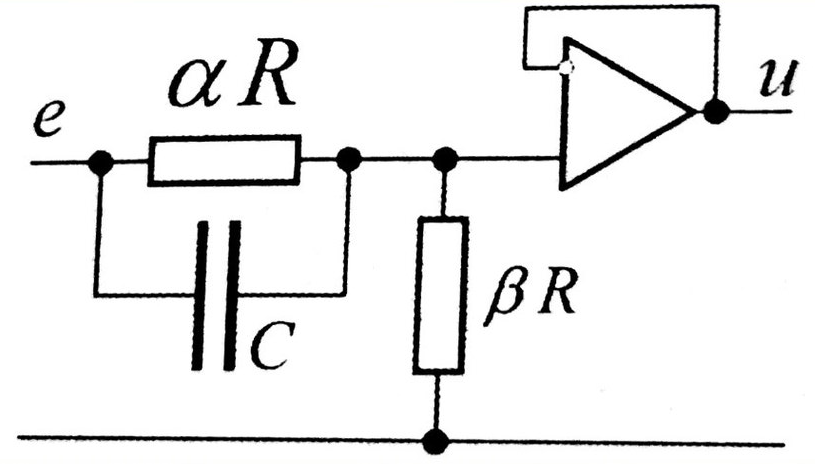
\includegraphics[width =  0.8\linewidth]{dif}
			\caption{Пропорционально дифференцирующее звено.}
	\end{figure}
\end{minipage}
~
\begin{minipage}[\right]{0.4\linewidth}
	\begin{figure}[H]
			\centering
			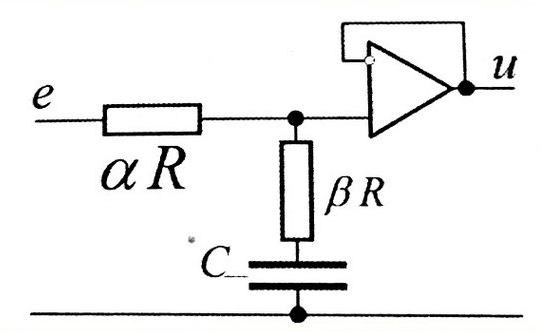
\includegraphics[width =  0.8\linewidth]{int}
			\caption{Пропорционально интегрирующее звено.}
	\end{figure}
\end{minipage}

~
\vspace{\baselineskip}

\textbf{1}. Измерим уровни подавления на частоте $f_0$ и в полосах задержания для пропорционально интегрирующей и дифференцирующей цепей с полюсом в точке $s = \frac{p}{\omega_0}= -1,~ f_0 = \frac{\omega_0}{2\pi} = 10k$ и нулями в точках $s=-2,~s=-\frac{1}{2}$.  Измерим уровни подавления на частоте $f_0$ и в полосах задержания.



$$\delta = \dfrac{\beta}{\alpha+\beta} = \dfrac{1}{2}-\text{уровень подавления в полосе задержания}$$

Подавление на частоте $f_0 = 10k$:
$$\dfrac{4}{5} - \text{интегрирующее звено},~\dfrac{1}{5} - \text{дифференцирующее звено}$$



~

\textbf{2}. Изменим номиналы резисторов в схемах так, чтобы сохранив положения полюсов, переместить нули в точки $s=-4,~s=-\frac{1}{4}$

$\delta = \frac{1}{4}$ - уровень подавления в полосе задержания.
Уровень подавления на частоте $f_0$: $\frac{1}{2}$ - интегрирующая, $\frac{3}{20}$ - дифференцирующая.

~

\textbf{3}. Откроем модель \textbf{integrator.cir} реального интегратора с частотой единичного усиления $f_1 = \frac{1}{2\pi RC} = 10k$ и усилением $K = \frac{R_K}{R}$.

\begin{minipage}{0.35\linewidth}
\begin{table}[H]
	\centering
	\begin{tabular}{c|cccccc}\toprule
		$f_1,~\text{Гц}$ & 10k & 10k  & 10k   & 10k   & 10k   & 10k   \\
		$K$              & 2   & 4    & 8     & 16    & 32    & 64    \\
		$f_0,~\text{Гц}$ & 5k  & 2.5k & 1.25k & 0.62k & 0.31k & 0.16k \\ \bottomrule
	\end{tabular}
\end{table}
\end{minipage}
~
\begin{minipage}{0.2\linewidth}
$ \; $



\end{minipage}
~
\begin{minipage}[R]{0.35\linewidth}
	\begin{figure}[H]
		\centering
		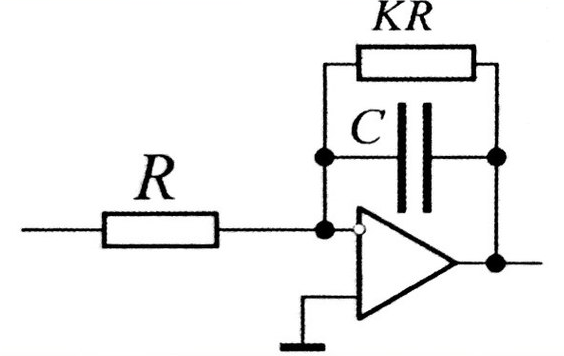
\includegraphics[width =  0.8\linewidth]{rint}
		\caption{Реальный интегратор.}
	\end{figure}
\end{minipage}

$\Longrightarrow f_1 = f_0K$ - соотношение выполняется.



\newpage
\section*{Задание №2. Активные звенья с двойным Т-мостом.}
\begin{figure}[H]
	\centering
	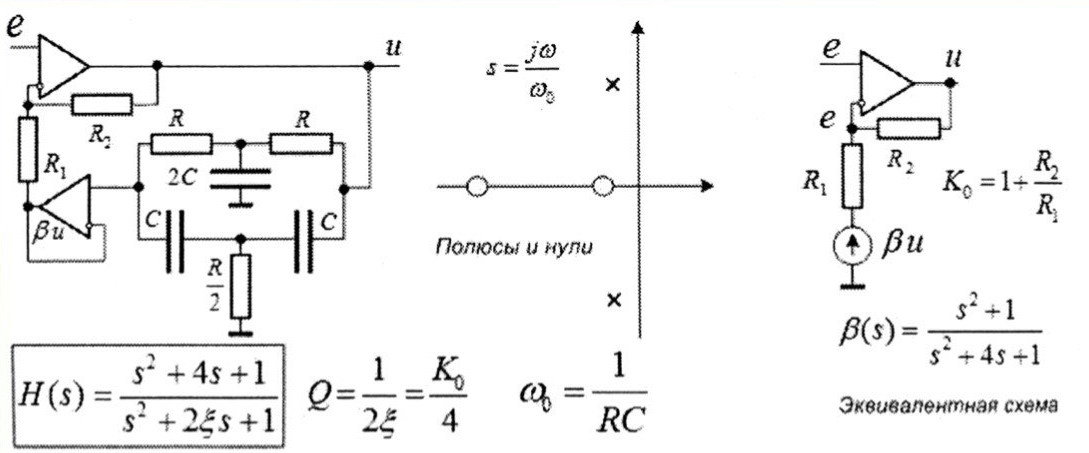
\includegraphics[width =  0.9\linewidth]{pfiltr}
	\caption{Полосовой фильтр с двойным Т - мостом.}
	\label{nus}
\end{figure}


\textbf{1}. Откроем модель полосового фильтра \text{pass2T.cir} с $f_0 = 10k,~ K_0 = 20$. Измерим усиление на частоте $f_0$ и полосу $\Delta f$ по уровню -3dB. Получаем $K_0 = 20.92,~\Delta f \hm{=} 1.93~(R_2 = 20k)$.

\begin{table}[H]
	\centering
	\caption{Зависимость пикового усиления и ширины полосы от $R_2$.}
	
	\begin{tabular}{c|cccc} \toprule
		$R_2,~\text{Ом}$      & 40k   & 60k   & 80k   & 100k   \\
		$K_0$      & 41.02 & 61.12 & 81.11 & 101.24 \\
		$\Delta f,~\text{Гц}$ & 979   & 643   & 495   & 397   \\ \bottomrule
	\end{tabular}
\end{table}

\textbf{2}.  Изучим поведение фильтра при разбалансировании моста варьированием $R_5$. Снимем зависимость от $R_5$ пикового усиления.

\begin{table}[H]
	\centering
	\caption{Зависимость пикового усиления от $R_5$.}
	
	\begin{tabular}{c|ccccccccc} \toprule
		$R_5,~\text{Ом}$ & 1.5   & 2     & 2.5   & 3      & 3.5   & 4     & 4.5   & 5     & 5.5   \\
		$K_0$            & 32.45 & 43.76 & 79.67 & 956.78 & 90.57 & 42.88 & 28.11 & 20.97 & 16.88 \\ \bottomrule
	\end{tabular}
\end{table}

\textbf{3}. Измерим уровни скачка в нуле и первого выброса: уровень скачка - $1$В при $R_5 = 5k~\text{Ом}$.

Оценим значение $R_5$, при котором фильтр теряет устойчивость.
\begin{table}[H]
	\centering
	\caption{Оценка $R_5$.}
	\begin{tabular}{c|cccccc} \toprule
		$R_5,~\text{Ом}$ & 5k   & 4.5k & 4k   & 3.5k & 3k   & 2.5k \\
		выброс           & 4.29 & 4.49 & 4.72 & 5.0  & 5.36 & 5.82 \\ \bottomrule
	\end{tabular}
\end{table}

Потеря устойчивости происходит при $R_5 = 3k~\text{Ом}$.

~

\textbf{4}. Откроем модель режекторного фильтра \textbf{stop2T.cir} с $f_0 = 10k,~\gamma = 0.1$.

\begin{figure}[H]
	\centering
	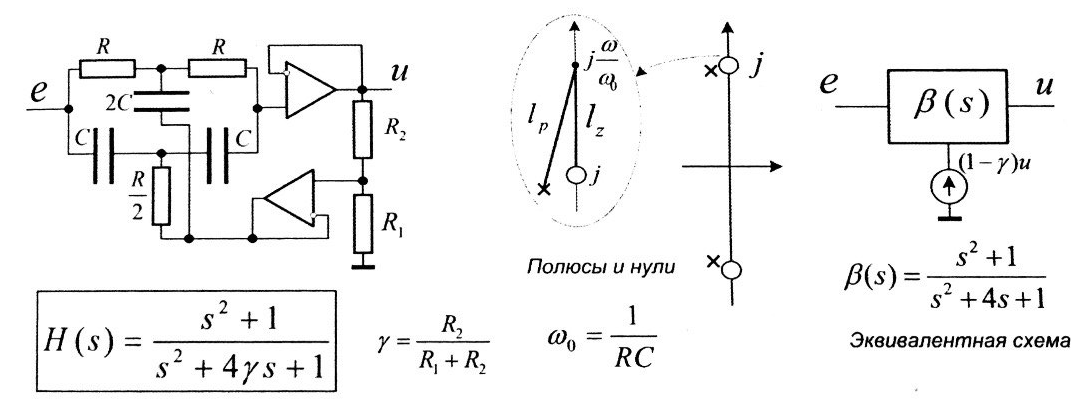
\includegraphics[width =  0.9\linewidth]{rfiltr}
	\caption{Режекторный  фильтр с двойным Т - мостом.}
	\label{nus}
\end{figure}

Измерим ширину полосы режекции $\Delta f$ по уровню $0.7 = -3 dB$. Получим: $\Delta f = 4.07~\text{кГц}$.

~

\textbf{5}. Измерим уровни скачка в нуле и первого выброса. Получим: уровень скачка - $1$В, первый выброс - $697.5$ мВ.

\newpage

\section*{Задание №3. Исследование созвездий.}
\textbf{2.} $ n =7,\; \varepsilon=1,\; \eta=2 \rightarrow \eta_1 = 5042$ --- уровень затухания фильтра Чебышева, тот же уровень затухания достигается фильтром Баттерворта порядка $ n=7 $ при $ \eta = 3.38 $

\textbf{3.} $ n=7,\; \varepsilon=1,\; \eta=1.5\rightarrow\eta_1=321.5 $ , порядок фильтра Баттерворта с тем же затуханием при $ \eta =1.5 \rightarrow \eta=15 $

\textbf{4.} Уровень затухания эллиптического фильтра при $ n=7,\;\varepsilon1,\;\eta=1.1 \rightarrow \eta_1=608.46 $. При селективности $ \eta=1.56  $ достигается тот же уровень затухания фильтром Чебышева $ n-7,\;\varepsilon=1 $

\textbf{7.} Полосовой фильтр с частотой $ f_0=465k $, двусторонней полосой $ \Delta f = 24k\left(Q=\frac{f_0}{\Delta f}\simeq20\right) $, неравномерностью 3dB($ \varepsilon=1 $) и затуханием $ \eta_1=10^4=80 $dB. Селективность $ \eta=1.36 $ обеспечивает затухание $ \eta_1 $ эллиптическим фильтром порядка $ n=7 $. При $ n=2 $ фильтр Чебышева обеспечивает сопоставимое значение селективности при том же затухании. Преобразовав эти фильтры в полосовые с $ Q=20 $ получаем максимальные добротности полюсов: $ Q_{max} = 1049.39 $ для эллиптического и $ Q_{max} = 2084.96 $ для фильтра Чебышева.

\newpage

\section*{Задание №4. Звенья Саллена-Ки.}

\begin{figure}[H]
	\centering
	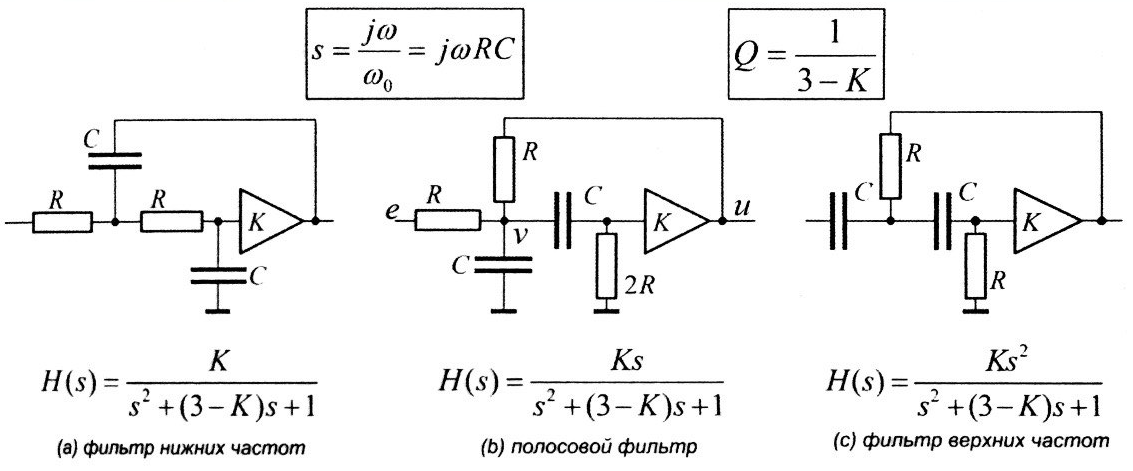
\includegraphics[width =  0.9\linewidth]{zvsk}
	\caption{Звенья Саллена-Ки.}
	\label{nus}
\end{figure}

\textbf{1}. Откроем модель \textbf{skey.cir} звеньев Саллена-Ки с частотой $f_0 = 10k$ и добротностью $Q = 1$. Измерим значения коэффициентов передачи при $f = f_0$. Получим:
$$K_0 = 2,~K_{lp} = 29.44,~ K_{hp} = 28.485,~K_{bp} = 28.898$$

\textbf{3.} Откроем модель \textbf{sk3pole.cir} с фильтрами Баттерворта верхних и нижних частот порядка $n = 3$ на частоту среза $f_0 = 10k$. Измерим скорости спада в $dB$ на октаву и затухания на частотах $f_0/2, ~ 2f_0$:

ВЧ: затухание на $f_0/2:-18~dB$, скорость спада  $-15 \frac{dB}{\text{дек}}$

НЧ: затухание на $2f_0: -18~dB$, скорость спада $15 \frac{dB}{\text{дек}}$.

~

Измерим уровни затухания фильтров Чебышева на частотах $f_0/2,~2f_0$:

ВЧ: затухание на $f_0/2:-30~dB$, скорость спада  $-18 \frac{dB}{\text{дек}}$

НЧ: затухание на $2f_0: -30~dB$, скорость спада $18 \frac{dB}{\text{дек}}$.

\textbf{4}. Откроем прототип \textbf{sk4pole.cir}, реализуем 4-полюсной полосовой фильтр Чебышева с $f_0 = 1k,~\epsilon = 1, Q = \frac{f_0}{\Delta f} = 6$. Измерим затухания на частотах $f_0/2,~2f_0,~f_0/10,~10f_0$.

\begin{table}[H]
	\centering
	\begin{tabular}{c|cccc} \toprule
		f         & $f_0/2$ & $2f_0$ & $f_0/10$ & 10f\_0 \\
		затухание & 1.83    & 1.75   & -27.9    & -27.9 \\ \bottomrule
	\end{tabular}
\end{table}
 
\newpage

\section*{Задание №5. Звенья с двойной обратной связью.}
\textbf{1.} Полосовое звено с $ f_0=5k,\; K_0=5,\;Q=15 $ 


\begin{minipage}{0.35\linewidth}
	\begin{figure}[H]
		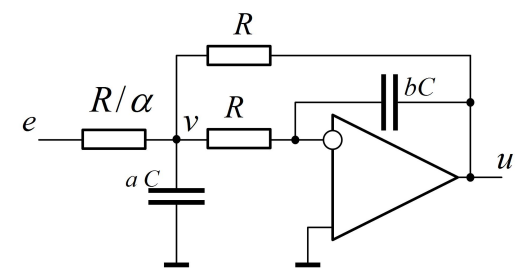
\includegraphics[width=60mm]{1}
	\end{figure} 
\end{minipage}
~
\begin{minipage}{0.65\linewidth}
	$ f_{max} = 4.980k, \Delta f=338 $ --- ширина полосы по уровню 0.7. $Q = \frac{f_{max}}{\Delta f} = 14.7,\; QK_0=73.5 $ --- пиковое усиление. 
\end{minipage}

\noindent Построим график зависимости частоты пика от $ R_2 $

\begin{minipage}{0.55\linewidth}
	\begin{table}[H]
		\begin{tabular}{c | c c c c c c c}
			$ R_2 $ & 100 & 300 & 500 & 700 & 900 & 1100 & 1300 \\ \midrule
			$ f $ & 12.7k & 7.6k & 6.1k & 5.3k & 4.7k & 4.4k & 4.1k 
		\end{tabular}
	\end{table}
\end{minipage}
~
\begin{minipage}{0.45\linewidth}
	\begin{figure}[H]
		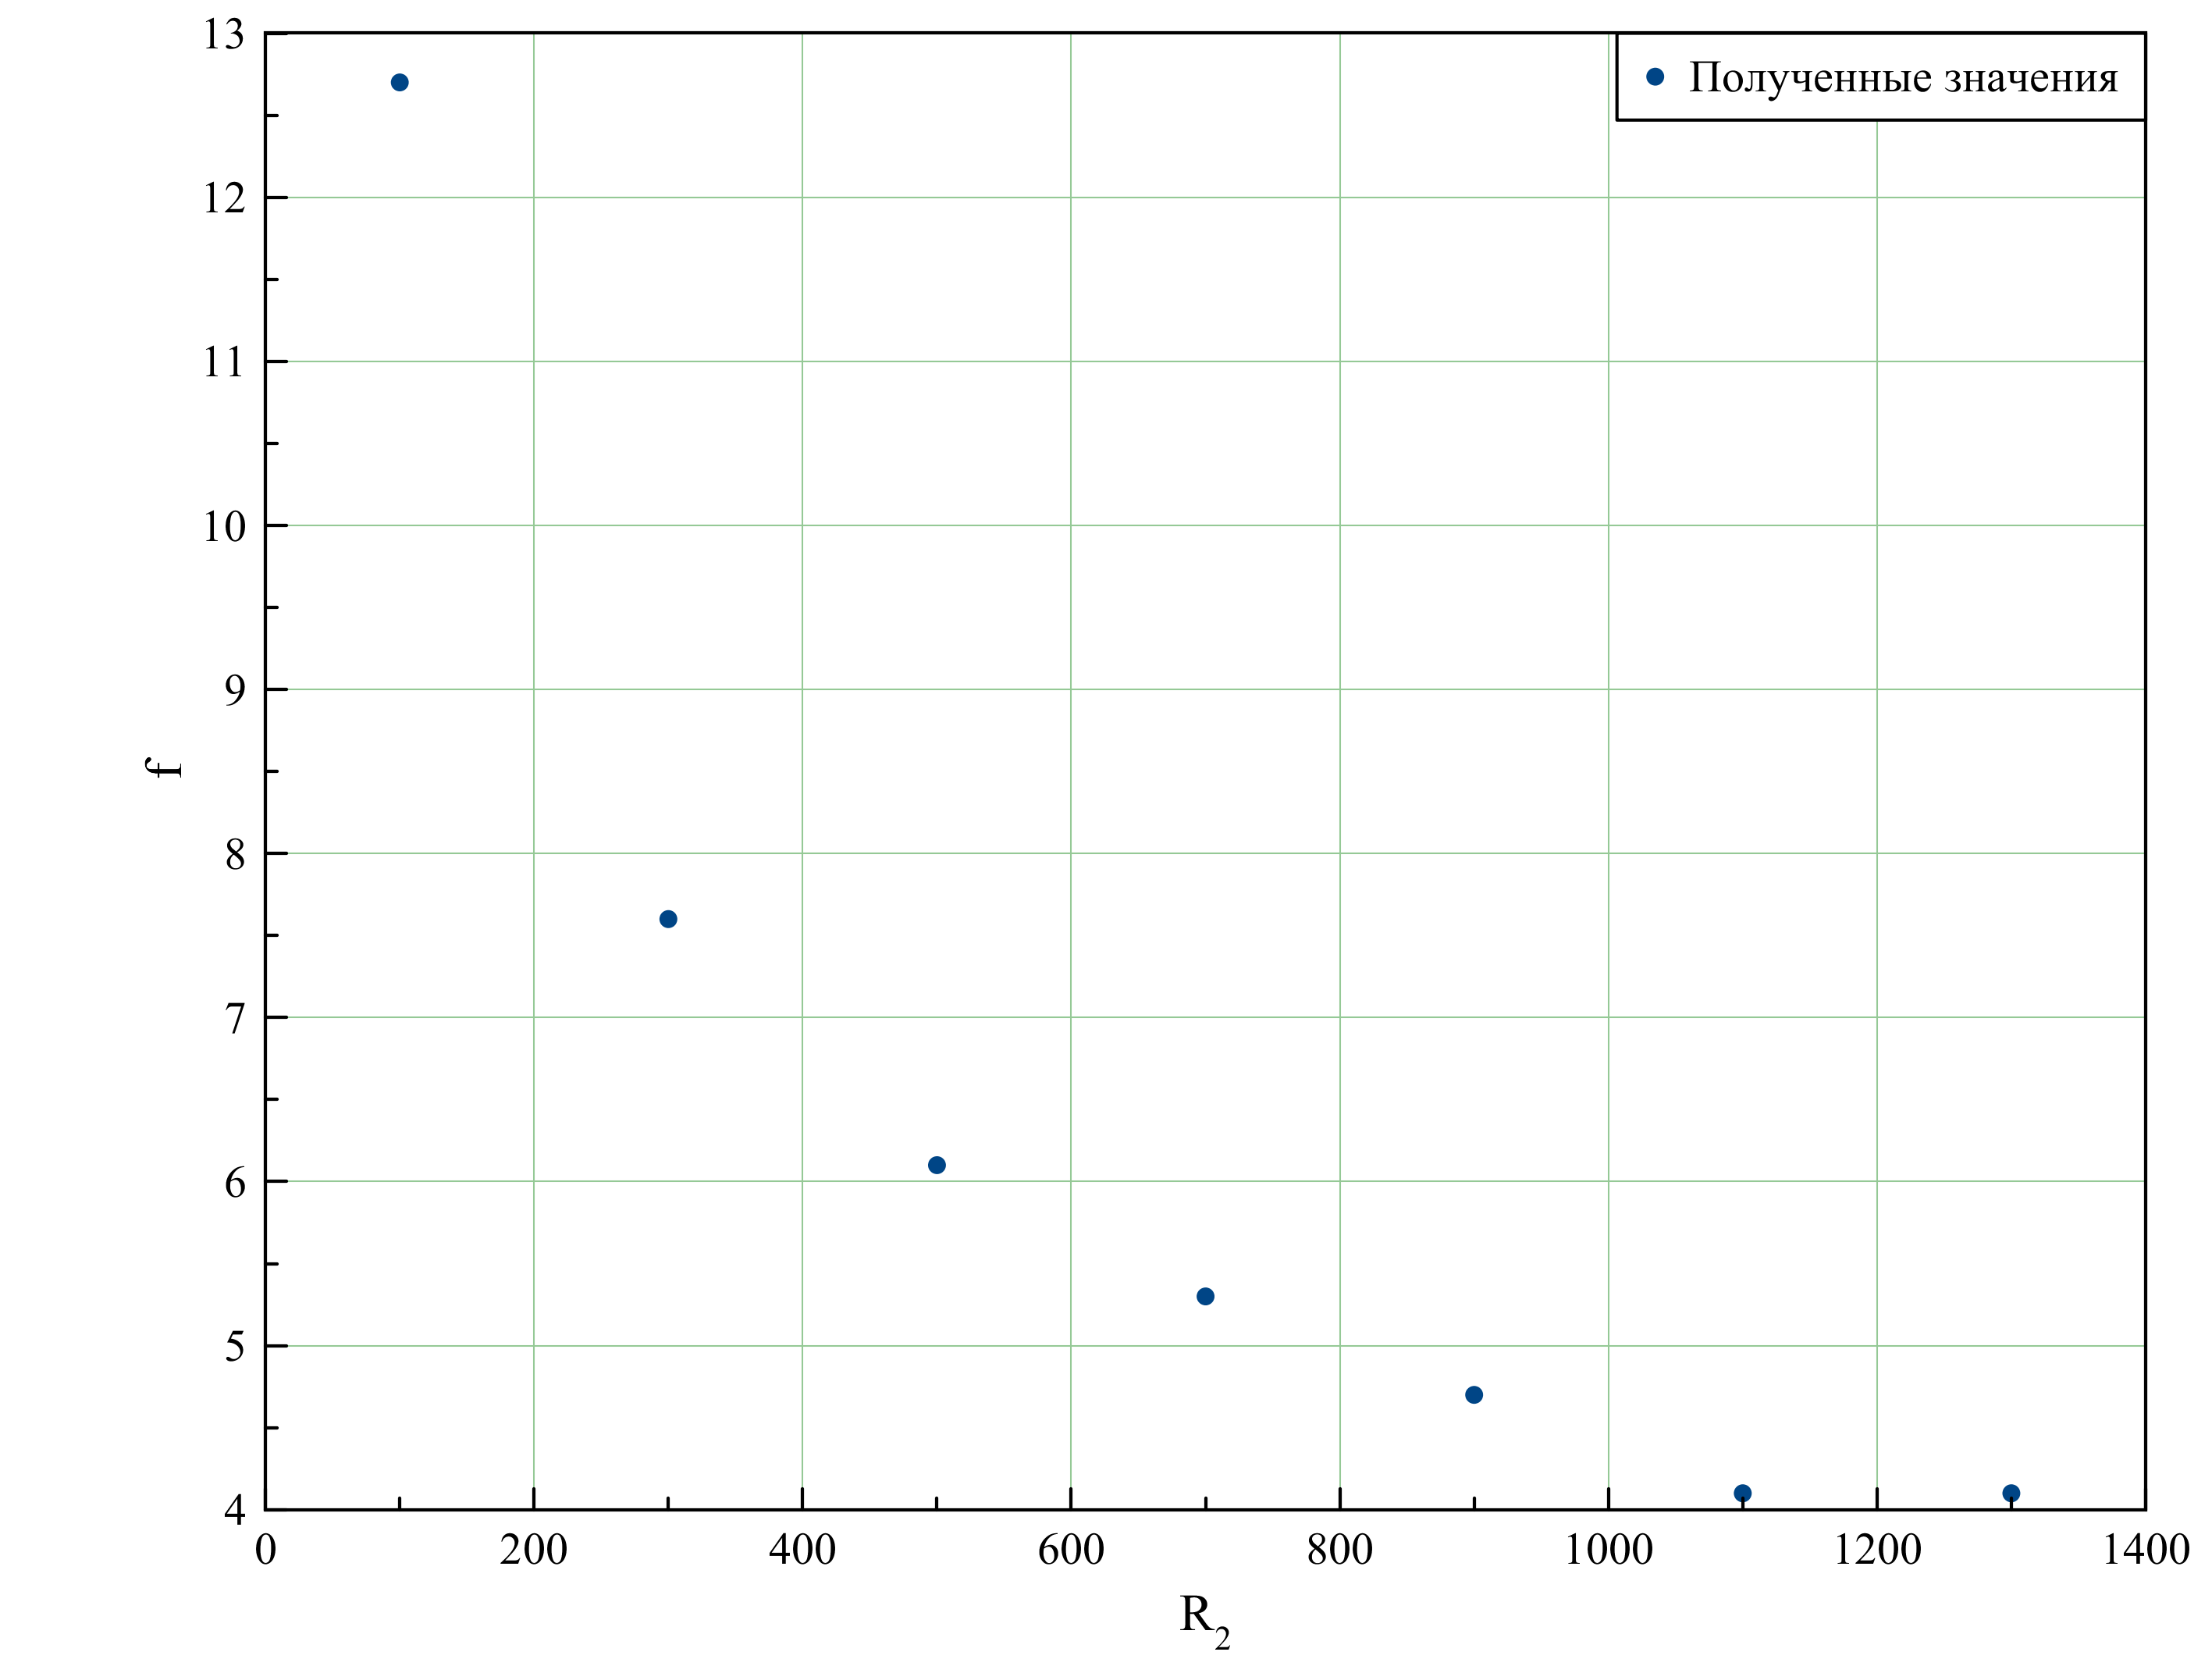
\includegraphics[width=70mm]{2}
	\end{figure}
\end{minipage}

\textbf{3.} $ C^* = С\nu_1 = 11.63 $ нФ, $ R^*=R/\nu_2 = 8.61 $ кОм. Затухания:
\begin{table}[H]
	\begin{tabular}{c | c c c}
		$ f $ & 0.5k & 2k & 10k \\ \midrule
		затухание & -7.88  & 1.28m & -26.3
	\end{tabular}
\end{table}

\newpage 

\section*{Задание №6. Полосовое звено на сдвоенном усилителе.}

\begin{figure}[H]
	\centering
	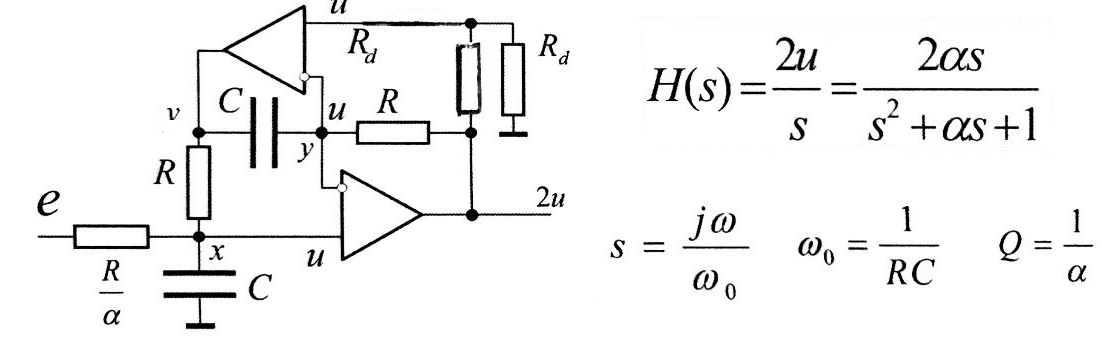
\includegraphics[width =  0.9\linewidth]{pfiltropus}
	\caption{Полосовой фильтр на сдвоенном операционном усилителе.}
	
\end{figure}

\textbf{1}. Откроем модель \textbf{amp2bp.cir}. По частотной характеристике звена оценим его параметры:$f_0 = 10k,~Q=9.7$. Измерим значение добротности при $R_2 = 6400k$.

~

\textbf{2}. Измерим частоту и уровень пика при $R_5 = 1.11k ~ (\gamma = \frac{R_5}{R_4+R_5} = 0.1)$: $f = 31.415k$, уровень пика - $24.079$.

\newpage

\section*{Задание №7. Звенья эллиптических фильтров.}
\textbf{1}. Реализуем трехполюсной эллиптический фильтр нижних частот с параметрами $ \eta \hm{=} 1.5,\; f_0=1k,\; \epsilon=1,\; \eta_1 = 35.61,\; \nu_z = 1.67512,\; \nu_0=0.34797,\;\nu_p=0.94016 $, затухание  — 31.03 dB	


Измерим границу $\eta$ полосы задержания, положение нуля и уровень затухания $\eta_1$:
$$ \epsilon = 0.64 ~\text{- неравномерность},  \eta = 1.478k~\text{ - граница полосы задержания}$$
$$ \eta_1 = 3.16~\text{- уровень затухания}, \text{положение нуля:}~ 1.672k $$
 \begin{figure}[H]
	\centering
	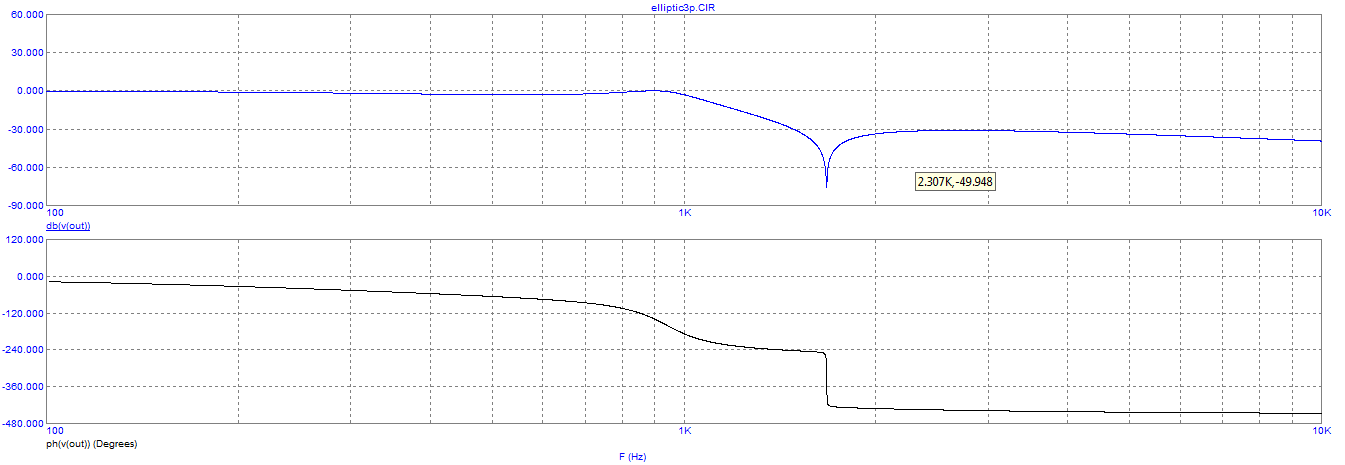
\includegraphics[width =  0.9\linewidth]{7i}
	\caption{АЧХ и ФЧХ фильтра нижних частот.}
	
\end{figure}

\textbf{2}. Реализуем фильтр верхних частот с теми же параметрами. Измерим границу $\eta$ полосы задержания, положение нуля и уровень затухания.
 $$ \varepsilon=0.59,\; \eta = 663.68,\; \eta_1 = 10.04 $$
 \begin{figure}[H]
 	\centering
 	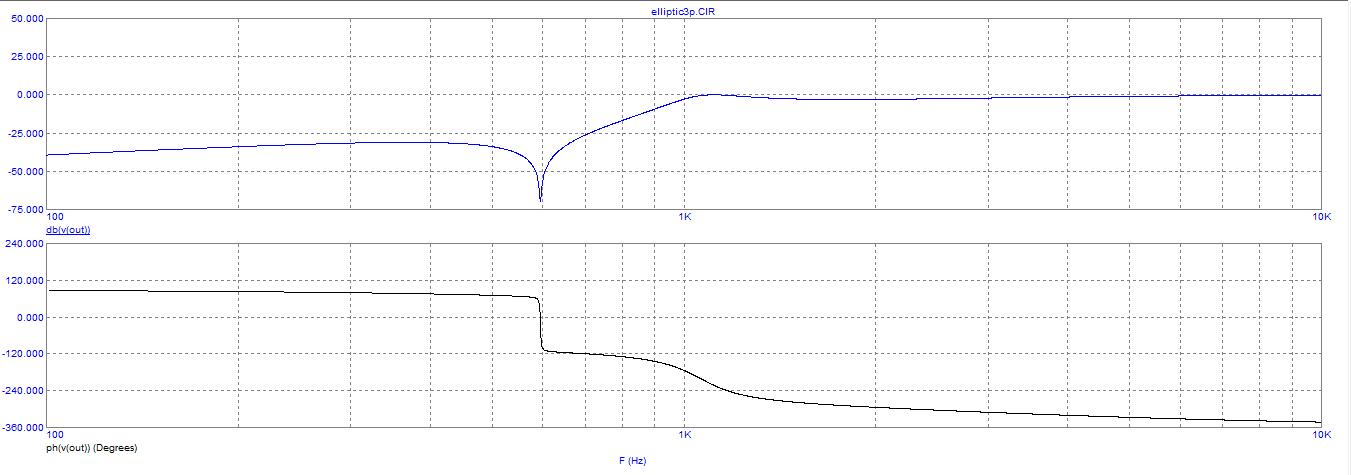
\includegraphics[width =  0.9\linewidth]{7d}
 	\caption{АЧХ и ФЧХ фильтра верхних частот.}
 	
 \end{figure}



\end{document}
